\documentclass[a4paper,twocolumn,10pt]{article}


%%\usepackage[english]{babel}
\usepackage[utf8]{inputenc}

\usepackage{graphicx} % figuras
\usepackage{subfigure} % subfiguras
\usepackage{amsmath}
\usepackage{algorithm}

\usepackage[noend]{algpseudocode}
%%\newcommand{\kw}[1]{\textrm{#1}}
\usepackage{comment}

%opening

\title{Análisis del algoritmo Dijkstra usando Binomial y Fibonacci Heap }
\author{Luigy Machaca Arcana\\Gabriel Aparicio Tony\\Universidad Nacional de San Agustín 
	\\ Escuela Profesional de Ciencia de la Computación 
	\\ Análisis y diseño de algoritmos}

%%/////////////////////////////////////////////////////////

\begin{document}


\twocolumn[
\begin{@twocolumnfalse}
\maketitle
~\newline
~\newline
~\newline
\begin{abstract}
Los heaps son estructuras de datos de prioridad de cola, en dónde 
la extracción del elemento (máximo o mínimo) es siempre $\theta(1)$.
Existen distintas formas de implementar este tipo de estructuras, algunas de estas son
binomial y los fibonacci heap. En el artículo se analizará algunas definiciones preliminares sobre dijkstra,
binomial heap y fibonacci heap, asi como se experimentará acelerando el algoritmo dijkstra con binomial 
y fibonacci heap respectivamente. También incluye los resultados y conclusiones de un experimento 
realizado para reforzar el análisis previo.
~\newline
~\newline
~\newline
~\newline
~\newline
~\newline
\end{abstract}
\end{@twocolumnfalse}
]


\section{Introducción}
Muchas veces necesitamos usar estructuras parcialmente ordenadas para recurrir al o a los elementos 
con mayor prioridad. Por ejemplo para el algoritmo de Dijkstra es necesario tener acceso inmediato 
a la arista con menor peso, por lo que las aristas deben estar almacenadas en una estructura 
parcialmente ordenada. Otro caso se da cuando queremos rankear los elementos, 
de tal forma que podemos obtener un top 5, top 10, etc. ya que solo nos 
importaría los primeros elementos. \\
Así como estas aplicaciones, existen muchas otras que necesitan 
de estructuras parcialmente ordenadas. Entre este tipo de estructuras se encuentran las priority queues, 
tales como listas enlazadas, binary heaps, binomial heaps, fibonacci heaps, relaxed heaps, etc. \cite{princeton_slides_binomial}.\\

Por otra parte Dijkstra es un algoritmo el cual partiendo de un nodo inicial, encuentra todos los caminos mas cortos,
hacialos demás nodos.

El objetivo de este articulo es analizar los algortimos de dijkstra (\ref{alg:dijkstra}) sin mejora alguna, 
segundo dijkstra con mejora de un heap binomial (\ref{alg:dijkstra_con_heap}) 
y tercero con mejora de un heap fibonacci (\ref{alg:dijkstra_con_heap}).

\section{Conceptos preliminares}

\subsection{Priority Queue}
\emph{Priority Queue es una estructura de datos fundamental que permite el acceso 
solo al elemento mínimo o máximo } \cite{libro_cormen} (según sea el orden). 
Una implementación de las priority queue es el Heap. Deben soportar por lo menos 
las siguientes operaciones: Insertar, Encontrar menor o mayor, Eliminar menor o mayor.
\subsection{Heap}
Un Heap es una estructura de datos especializada basada en el concepto de árbol, que satisface la 
siguiente propiedad: Para todo nodo A cuyo padre es P, A debe estar ordenado respecto a P.
Entre algunos tipos de Heap estan: Binary Heap, \textbf{Binomial Heap}, \textbf{Fibonacci Heap}, Radix Heap, 
d-ary Heap, Soft Heap, etc. El Min-Max Heap es un caso especial, ya que deja de ser un árbol.

\subsection{Binomial Heap}
BINOMIAL TREE: Un árbol binomial es un árbol ordenado definido recursivamente, como sigue:
Sea $B_k$ un árbol binomial
\begin{itemize}
\item $B_0$ es un sólo nodo
\item Para $k>0$ , $B_k$ consiste en dos $B_(k-1)$'s que están unidos entre sí de manera 
que la raíz de uno es el hijo izquierdo de la raíz de la otra
\end{itemize}

Un Binomial Heap es un conjunto de árboles binomiales tales que:
\begin{itemize}
  \item Cada árbol binomial es un árbol parcialmente ordenado, es decir la clave de todo nodo es mayor(menor) o igual que la de su padre. 
  \item Contiene no más de un árbol binomial $B_i$ para cada grado $i$
\end{itemize}
La mayoría de operaciones del binomial heap están basadas en la operación de unión. Este algoritmo 
utiliza dos funciones: Unión de dos árboles binomiales de un mismo grado y una operación mezclar, 
que se encarga de enlazar los nodos del primer nivel de dos heaps de acuerdo al orden de sus grados.
\newline
La operación de inserción utiliza la operación de unión, simplemente aplicándola al heap y a un nodo creado a 
partir de la llave. Un ejemplo es la figura \ref{Figure:binomial_heap}.

\begin{figure}
 \caption{Ejemplo de Árboles binomiales}\label{Figure:binomial_heap}
 \centering
    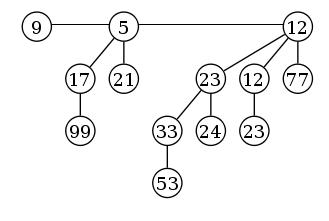
\includegraphics[width=0.3\textwidth]{binomial_heap.jpg}
\end{figure}

\subsection{Fibonacci heap}

 Es una coleccion de árboles que satisfacen la propiedad del del min-heap. \cite{princeton_slides_rezaul_dijkstraFibonacci}

\begin{itemize}
\item es similar a un Binomial-Heap, pero es una estructura menos rigida
\item Un Binomial-Heap al insertar ordena tus nodos, un Fibonacci-Heap no lo hace
\item Fibonacci solo ordena sus nodos, cuando delete-min es llamado
\item Tiene una funcion potencial: $\varphi(H) = tree(H)+2*marks(H)$
\end{itemize}

A diferencia del Binomial-Heap, la mayoría de operaciones no están basadas en la operación de unión. Este algoritmo 
solo usa la operacion Union-heap cuando Delete-min es llamado.
\newline
Un ejemplo es la figura \ref{Figure:fibonacci_heap}.

\begin{figure}
 \caption{Ejemplo de Árboles binomiales}\label{Figure:fibonacci_heap}
 \centering
    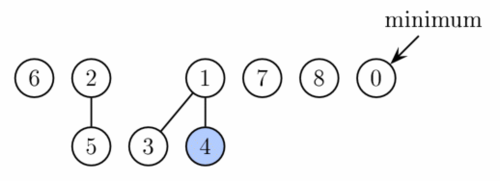
\includegraphics[width=0.4\textwidth]{fibonacci_heap.png}
\end{figure}


\subsection{Comparación Heap}
~\newline
En la siguiente tabla se compara el costo computacional en el peor caso de las principales funciones en cada. 
Heap \cite{libro_cormen}

\vspace{5mm}
~\newline
\begin{tabular}{ l | c | c }
 \hline                        
  Función & Fibonacci Heap& Binomial Heap\\
	  & (Peor caso) & (Peor Caso) \\
  \hline
  Insert & $(1)$ & $\log(n)$ \\
  Decrease key & $(1)$ & $(\log(n))$ \\
  Encontrar mínimo & $(1)$relajado & $(1)$relajado \\
  Extraer mínimo & $\log(n)$ & $\log(n)$ \\
  Union & $(1)$ & $(\log(n))$ \\
  \hline
\end{tabular} 


\subsection{Dijkstra}
También llamado \textbf{algoritmo de caminos minimos}, este algoritmo sirve para determinar el camino mas corto 
hacia todos los demas vertices, en otras palabras dado los vertices $(i) \epsilon  G$, donde $G$ representa 
los vertices del grafo, $!E$ un camino minimo $c$, de $i$ hacia $f$, para todo $(f)\epsilon G$-\{i\}.\\
Siendo la idea principal hallar todos lo caminos minimos de $i$ hacia todos los demas elemnento del grafo $G$.\\
En el algoritmo [\textbf{\ref{alg:dijkstra}}] se expone el pseudocódigo.

\begin{algorithm}
\caption{Algoritmo Dijkstra}\label{alg:dijkstra}
\begin{algorithmic}
    \Procedure{Dijkstra}{$G,a:$ G es un grafo bidireccional, $a$ es nodo incial }
			\Comment{ todos los pesos de las aristas son positivos }
    \For {$i=1$ \textbf{to} n}
      \State $L(v_i)=\inf$ 
      \EndFor
    \State $L(a)=0$
    \State $S=\O{}$
    \While{$z \notin S$} \Comment{z es un nodo ya visitado}
      \State $u=a$  \Comment{$a$ no es vertice de $S$ y es minimo $L(u)$ }
      \State $S=S \bigcup \{u\}$
      \For{todos los vertices $v \notin S$} \Comment{\textbf{extracción del minimo}}
	 \If{$L(u)+ W(u,v)< L(v)$}    
	    \State $L(v)=L(u)+W(u,v)$
	 \EndIf
	 \EndFor
    \EndWhile 
    \State \textbf{return} $L(z)$\Comment{retorna los caminos mas cortos}
\EndProcedure 
\end{algorithmic}
\end{algorithm}

~\newline 
Podemos notar que en el algoritmo [\textbf{\ref{alg:dijkstra}}] en la linea \textbf{$8$}, que la extracción
del minimo es \textbf{$O(v)$},siendo esta una busqueda secuencial. Es posible mejorar esta extracción usando algun \textbf{heap},
este algoritmo es mostrado en [\textbf{\ref{alg:dijkstra_con_heap}}], teniendo en este caso un tiempo del \textbf{extract-min}
del heap usado.

\subsubsection{compraciones}
\begin{itemize}
  \item \textbf{Dijkstra con busqueda secuencial}\\
	extract-min demora en $v$ vertices $O(v)$, sabiendo que extract-min se encuentra contenido en \textbf{while}
	convierte  este tiempo en $O(v^2)$, como existen $E$ adyacentes, entonces el bucle itera $E$ veces con $O(1)$,
	osea el tiempo tomado por el algoritmo es $O(v^2 + E)$, osea $O(V^2)$.
  \item \textbf{Dijkstra con binomial heap}\\
	insert en un binomial en $v$ vertices $O(log(v))$, como existen $E$ adyacentes, la inserción demora un total de
	$O(E*lg(v))$.
  \item \textbf{Dijkstra con fibonacci heap}\\
	insert en un fibonacci en $v$ vertices $O(1)$, como existen $E$ adyacentes, la inserción demora un total de
	$O(E*(1))$, osea $O(E)$.
\end{itemize}

%%%%%%%%%%%%%%%%%%%%%%%%%%%%%%%%%%%%%%%%%%%%%%%%%%%%%%%%%%%%5
\begin{algorithm}
\caption{Algoritmo Dijkstra}\label{alg:dijkstra_con_heap}
\begin{algorithmic}
    \Procedure{Dijkstra}{$G,a:$ G es un grafo bidireccional, $a$ es nodo incial }
			\Comment{ todos los pesos de las aristas son positivos }
    \For {$i=1$ \textbf{to} n}
      \State $L(v_i)=\inf$ 
      \EndFor
    \State $L(a)=0$
    \State $S=\O{}$
    \While{$z \notin S$} \Comment{z es un nodo ya visitado}
      \State $u=a$  \Comment{$a$ no es vertice de $S$ y es minimo $L(u)$ }
      \State $S=S \bigcup \{u\}$
      \State $L(v)=extraer_minimo de v \notin S $ \Comment{\textbf{extracción del minimo}}
	 \If{$L(u)+ W(u,v)< L(v)$}    
	    \State $L(v)=L(u)+W(u,v)$
	 \EndIf
    \EndWhile 
    \State \textbf{return} $L(z)$\Comment{retorna los caminos mas cortos}
\EndProcedure 
\end{algorithmic}
\end{algorithm}
%%%%%%%%%%%%%%%%%%%%%%%%%%%%%%%%%%%%%%%%%%%%%%%%%%%%%%%%%%%%%%%%%%%%%%%%%%5


\section{Experimentos}
\subsection{Especificación de Entorno}
Los experimentos se realizaron en una computadora con las siguientes características: Memoria de 7.8 GiB. 
Procesador: Intel Core i7-3770 CPU  @ 3.40GHz x 8
\newline
Los algoritmos se implementaron en el lenguaje de programación C++, sobre el Sistema Operativo Linux en la distribución Ubuntu 14.04 LTS 64-bit
\subsection{Resultados}
Los datos obtenidos sobre un grafo, son resultado de la inserción de $n$ vertices con 8 vertices aleatorios cado uno. 
Se utilizó la función $gettimeofday$ para calcular los tiempos de ejecución. 
Es necesario aclarar que se insertaron random pesos en las aristas. 
Los tiempos de ejecución fueron calculados en microsegundos.

~\newline
\begin{itemize}
 \item En la Figura (\ref{Figure:dijkstra}) se puede observar la gráfica de estos resultados de \textbf{Dijkstra sin cambios}.
 \item En la Figura (\ref{Figure:dijkstra}) se puede observar la gráfica de estos resultados de \textbf{Dijkstra con Binomial}.
 \item En la Figura (\ref{Figure:dijkstra}) se puede observar la gráfica de estos resultados de \textbf{Dijkstra con Fibonacci}.
\end{itemize}



\begin{figure}
 \caption{Resultados}\label{Figure:dijkstra}
 \subfigure[dijkstra]{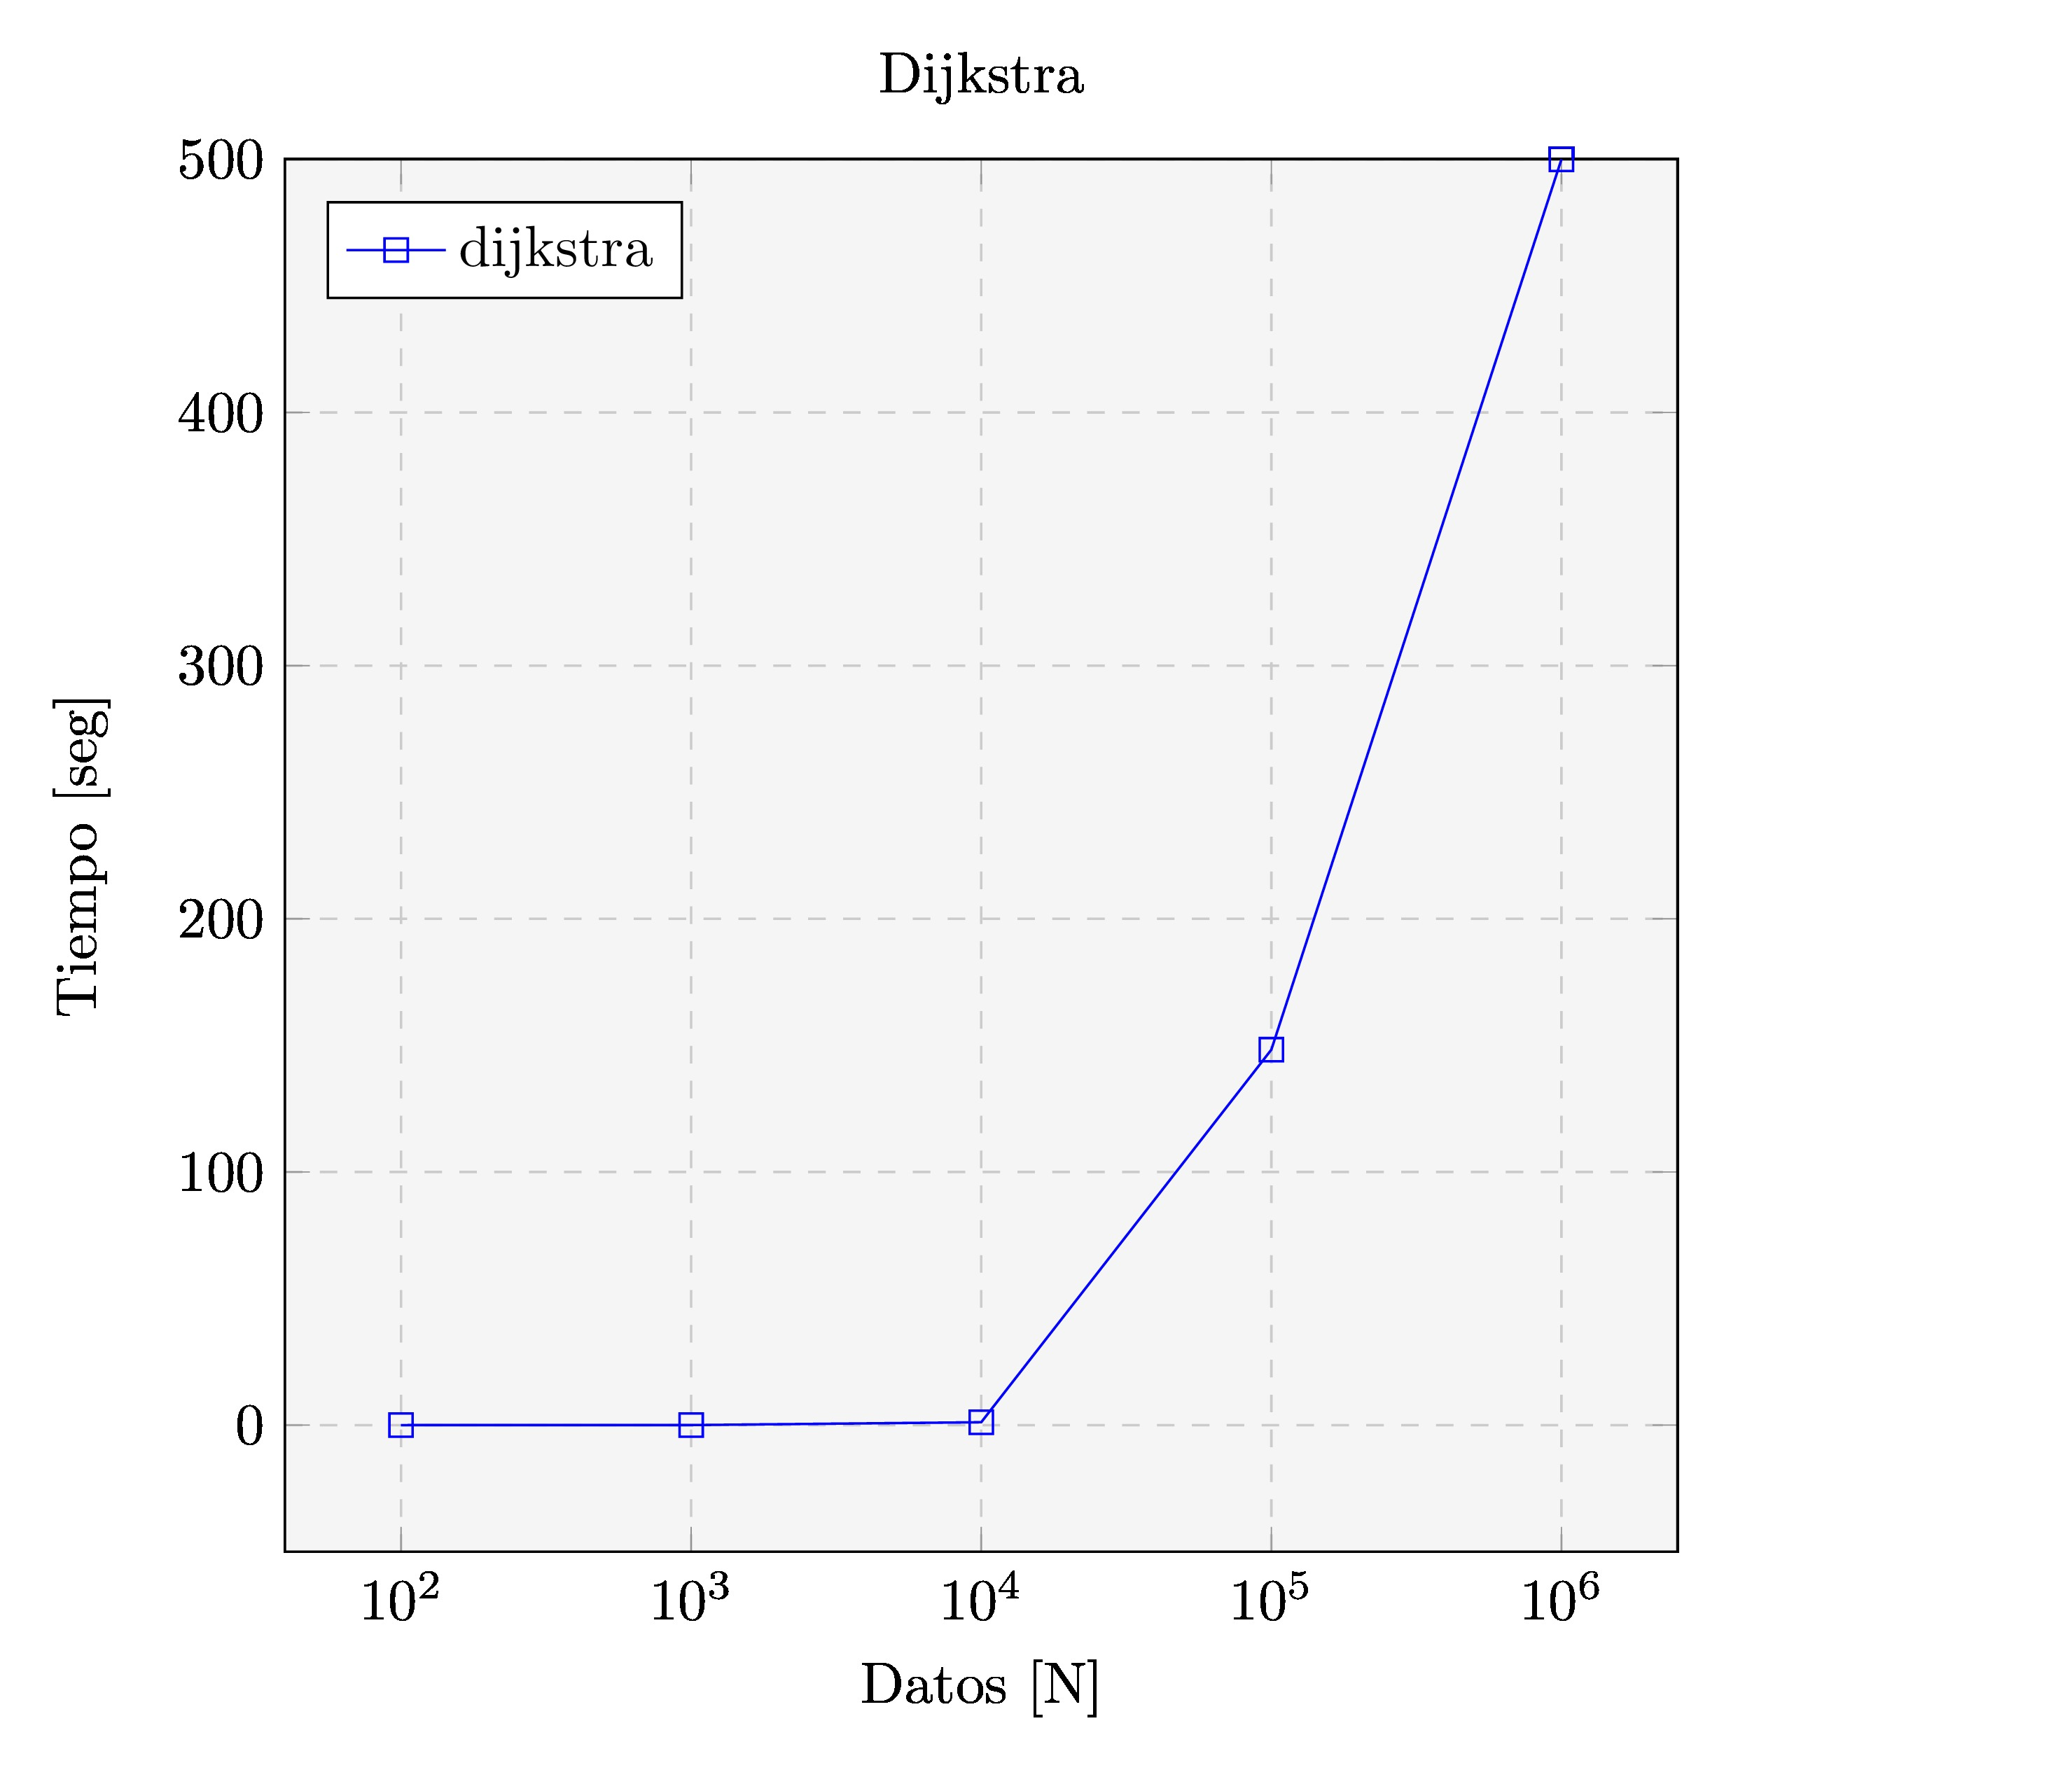
\includegraphics[width=0.5\textwidth]{graficos-0.jpg}}
 \subfigure[dijkstrabinomial]{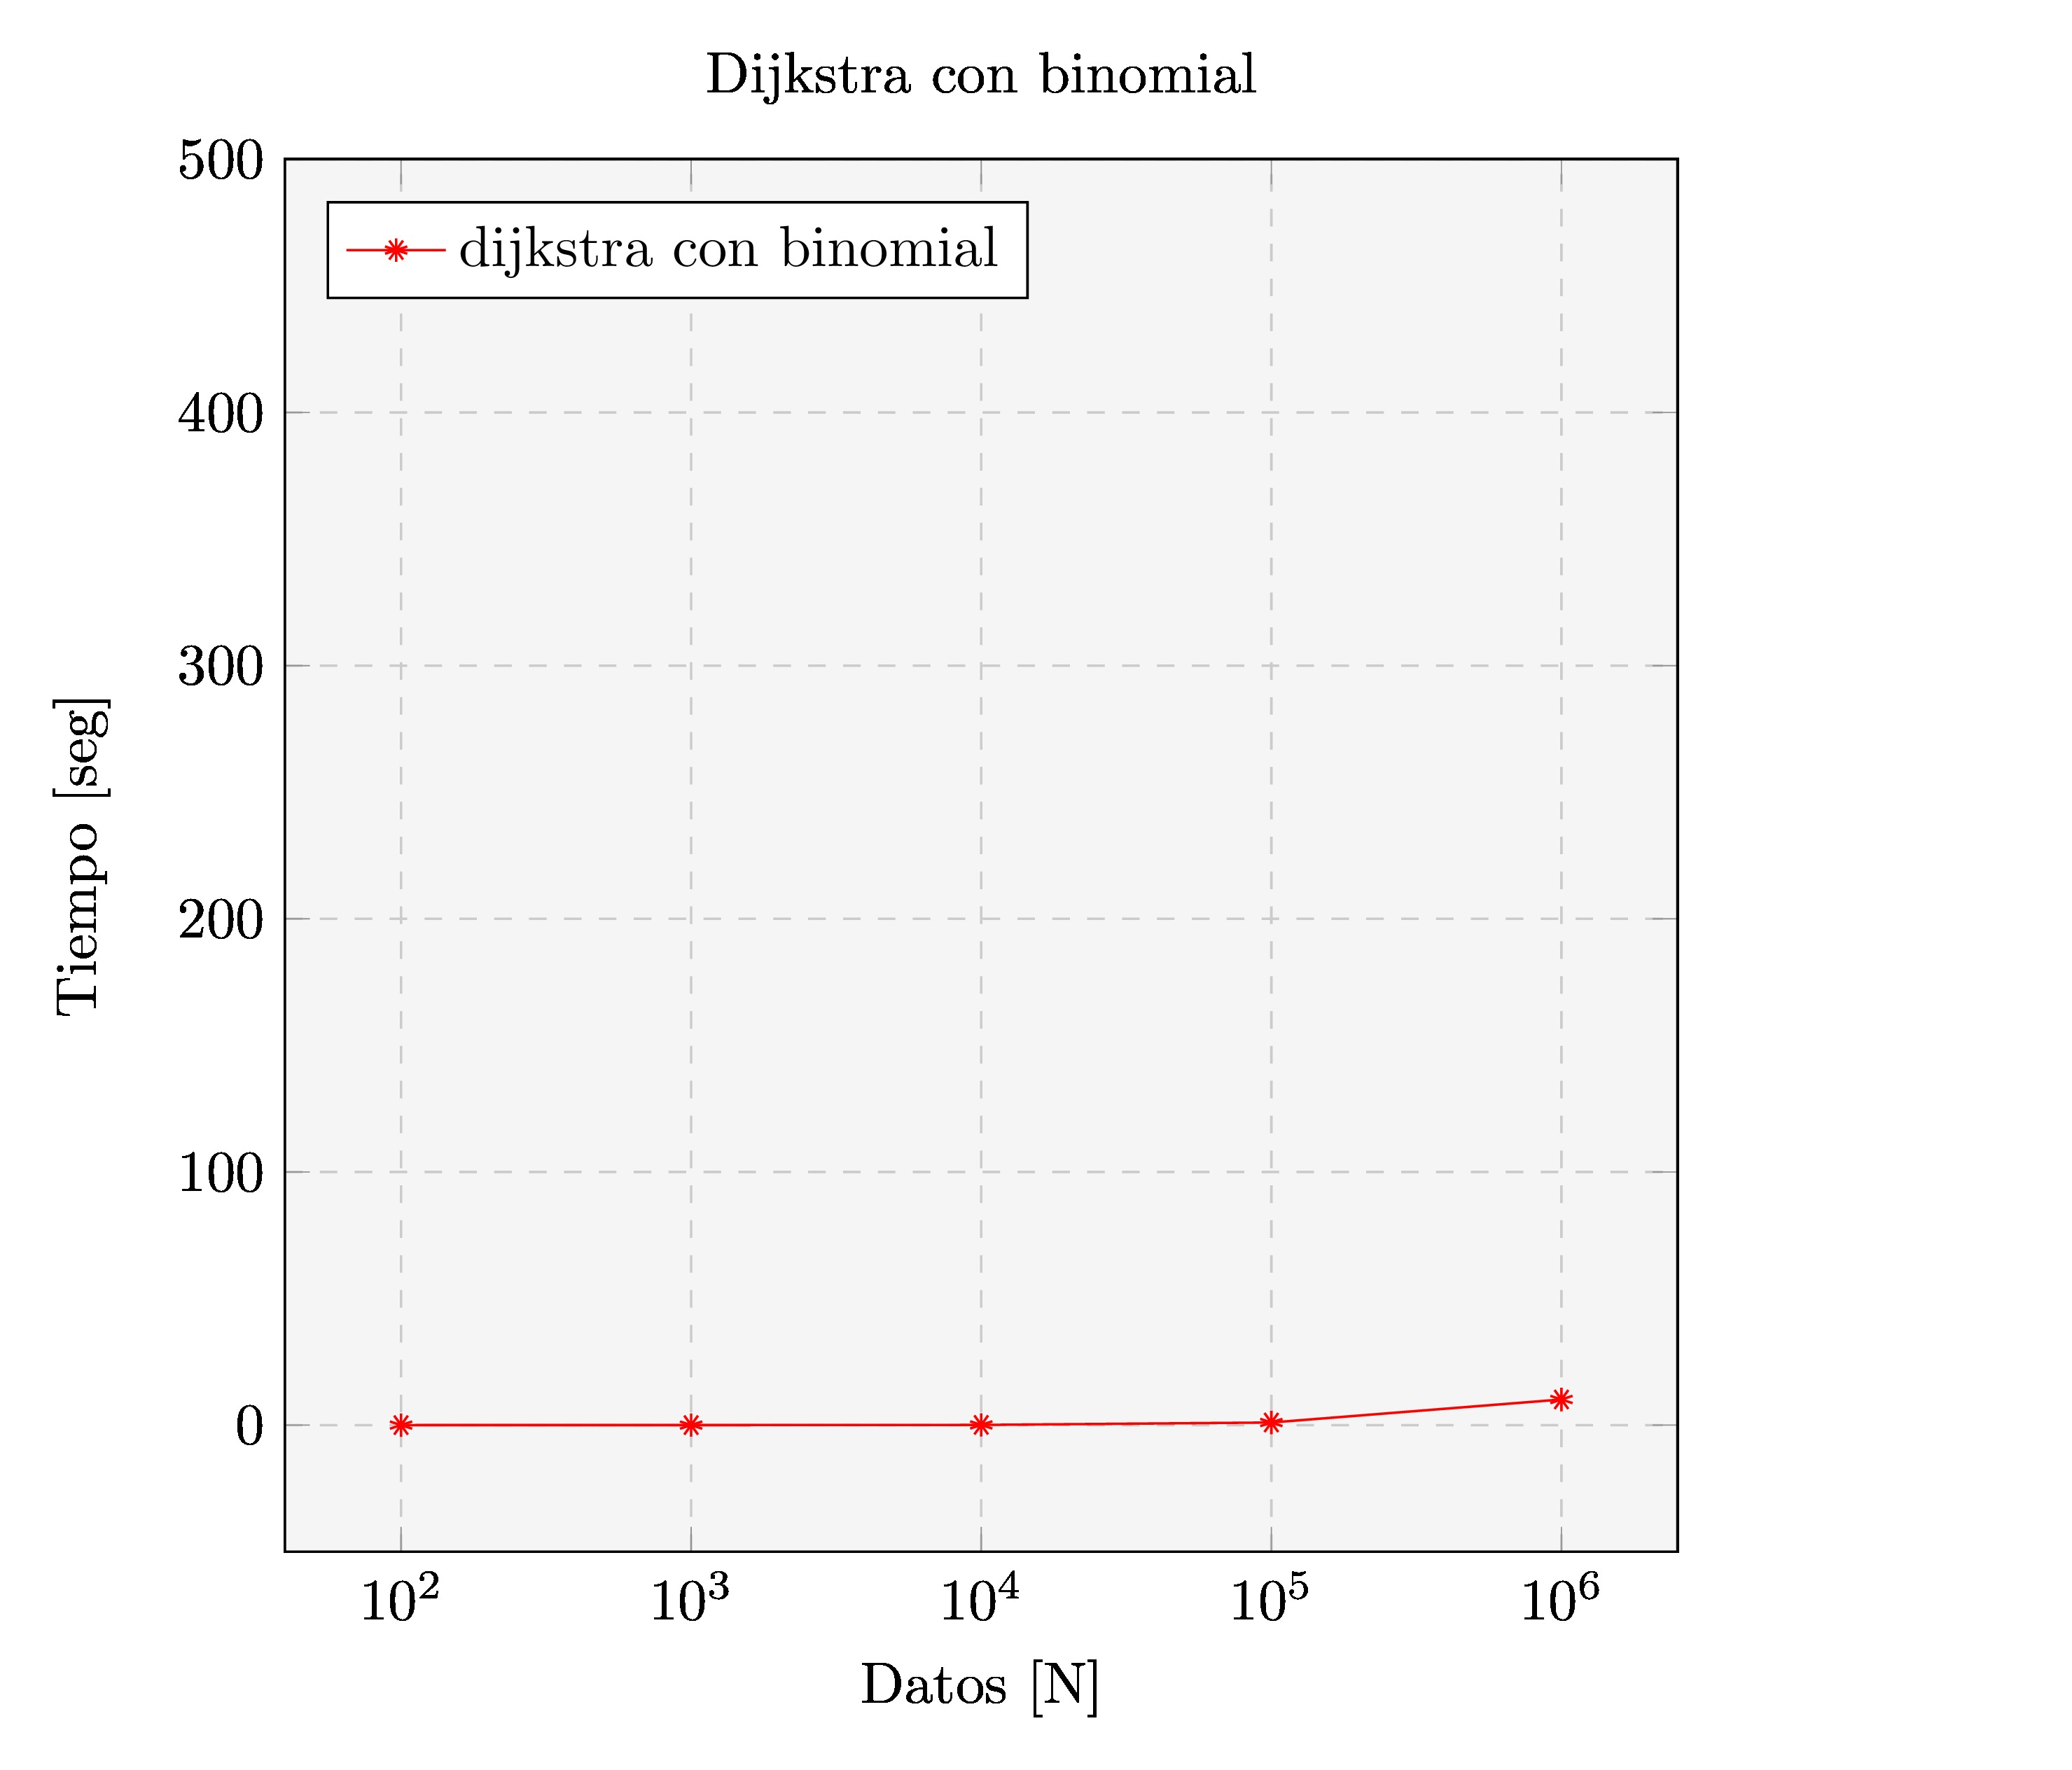
\includegraphics[width=0.5\textwidth]{graficos-1.jpg}}
 \subfigure[dijkstrafibonacci]{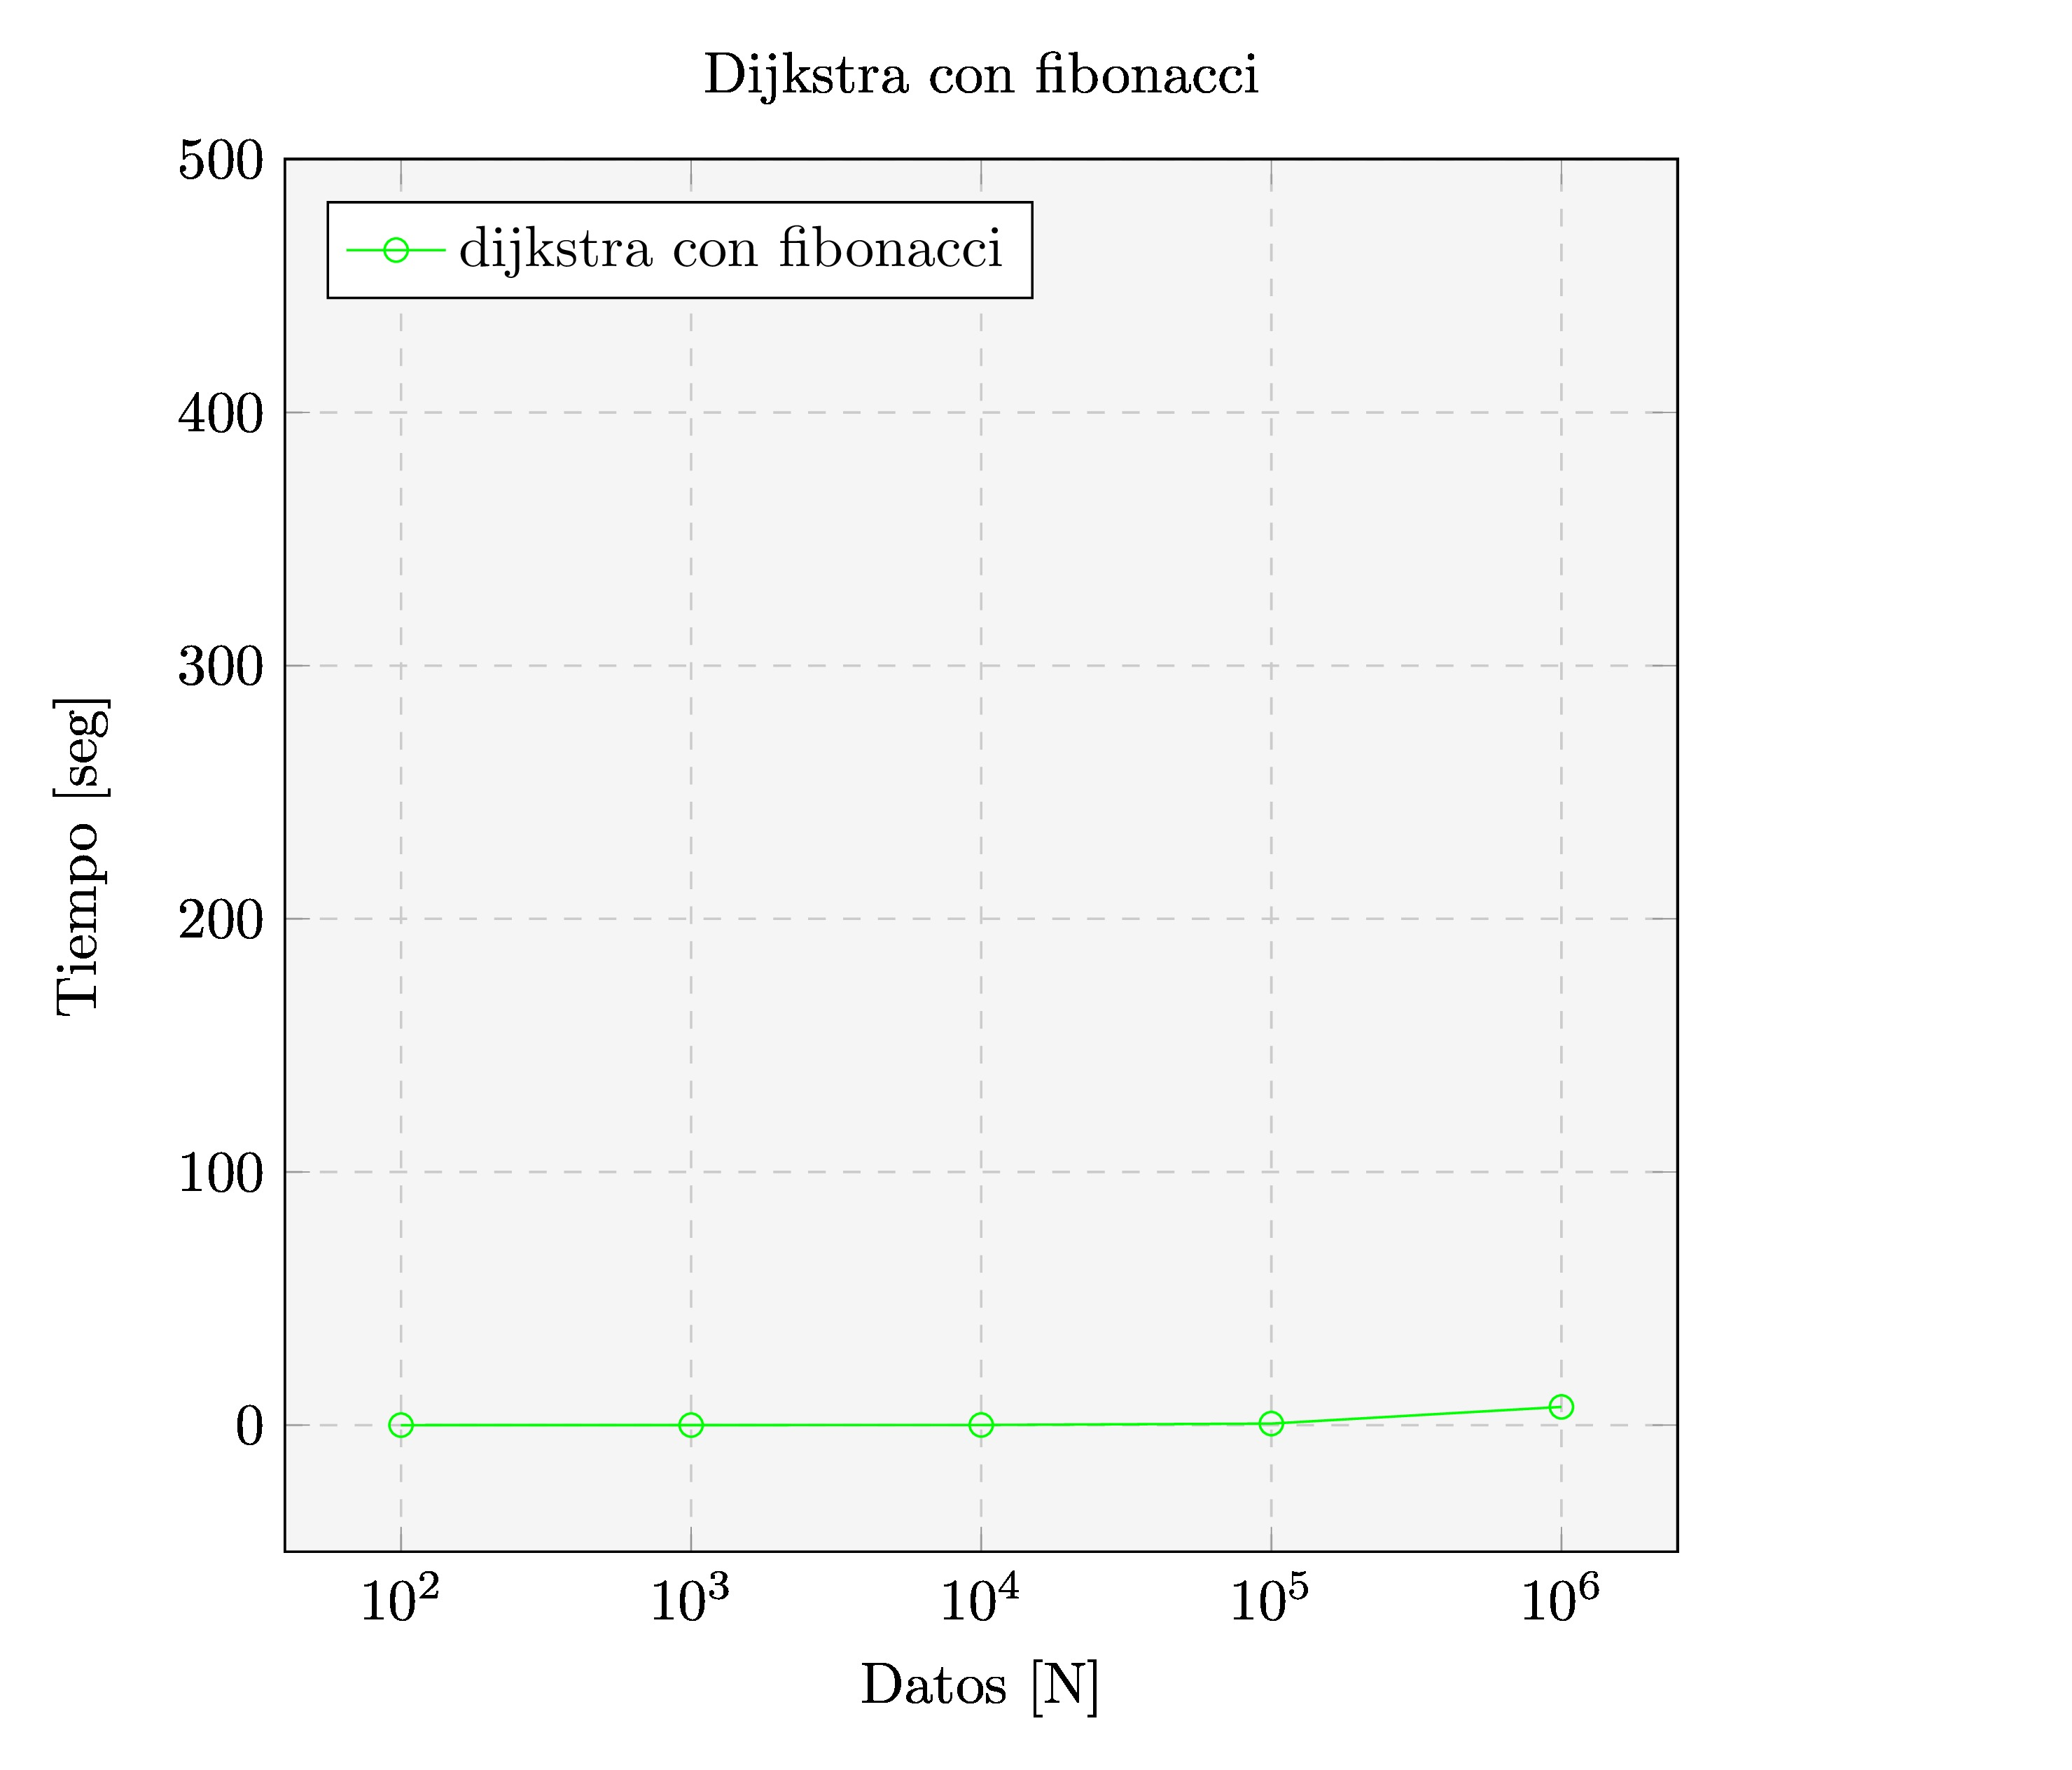
\includegraphics[width=0.5\textwidth]{graficos-2.jpg}}
 %\centering
    
\end{figure}


\begin{itemize}
 \item En la Figura (\ref{Figure:comparacion}) se puede observar la gráfica de estos resultados de \textbf{Comparacion de resultado}.
\end{itemize}

\begin{figure}
 \caption{compracion de resultados}\label{Figure:comparacion}
% \centering
    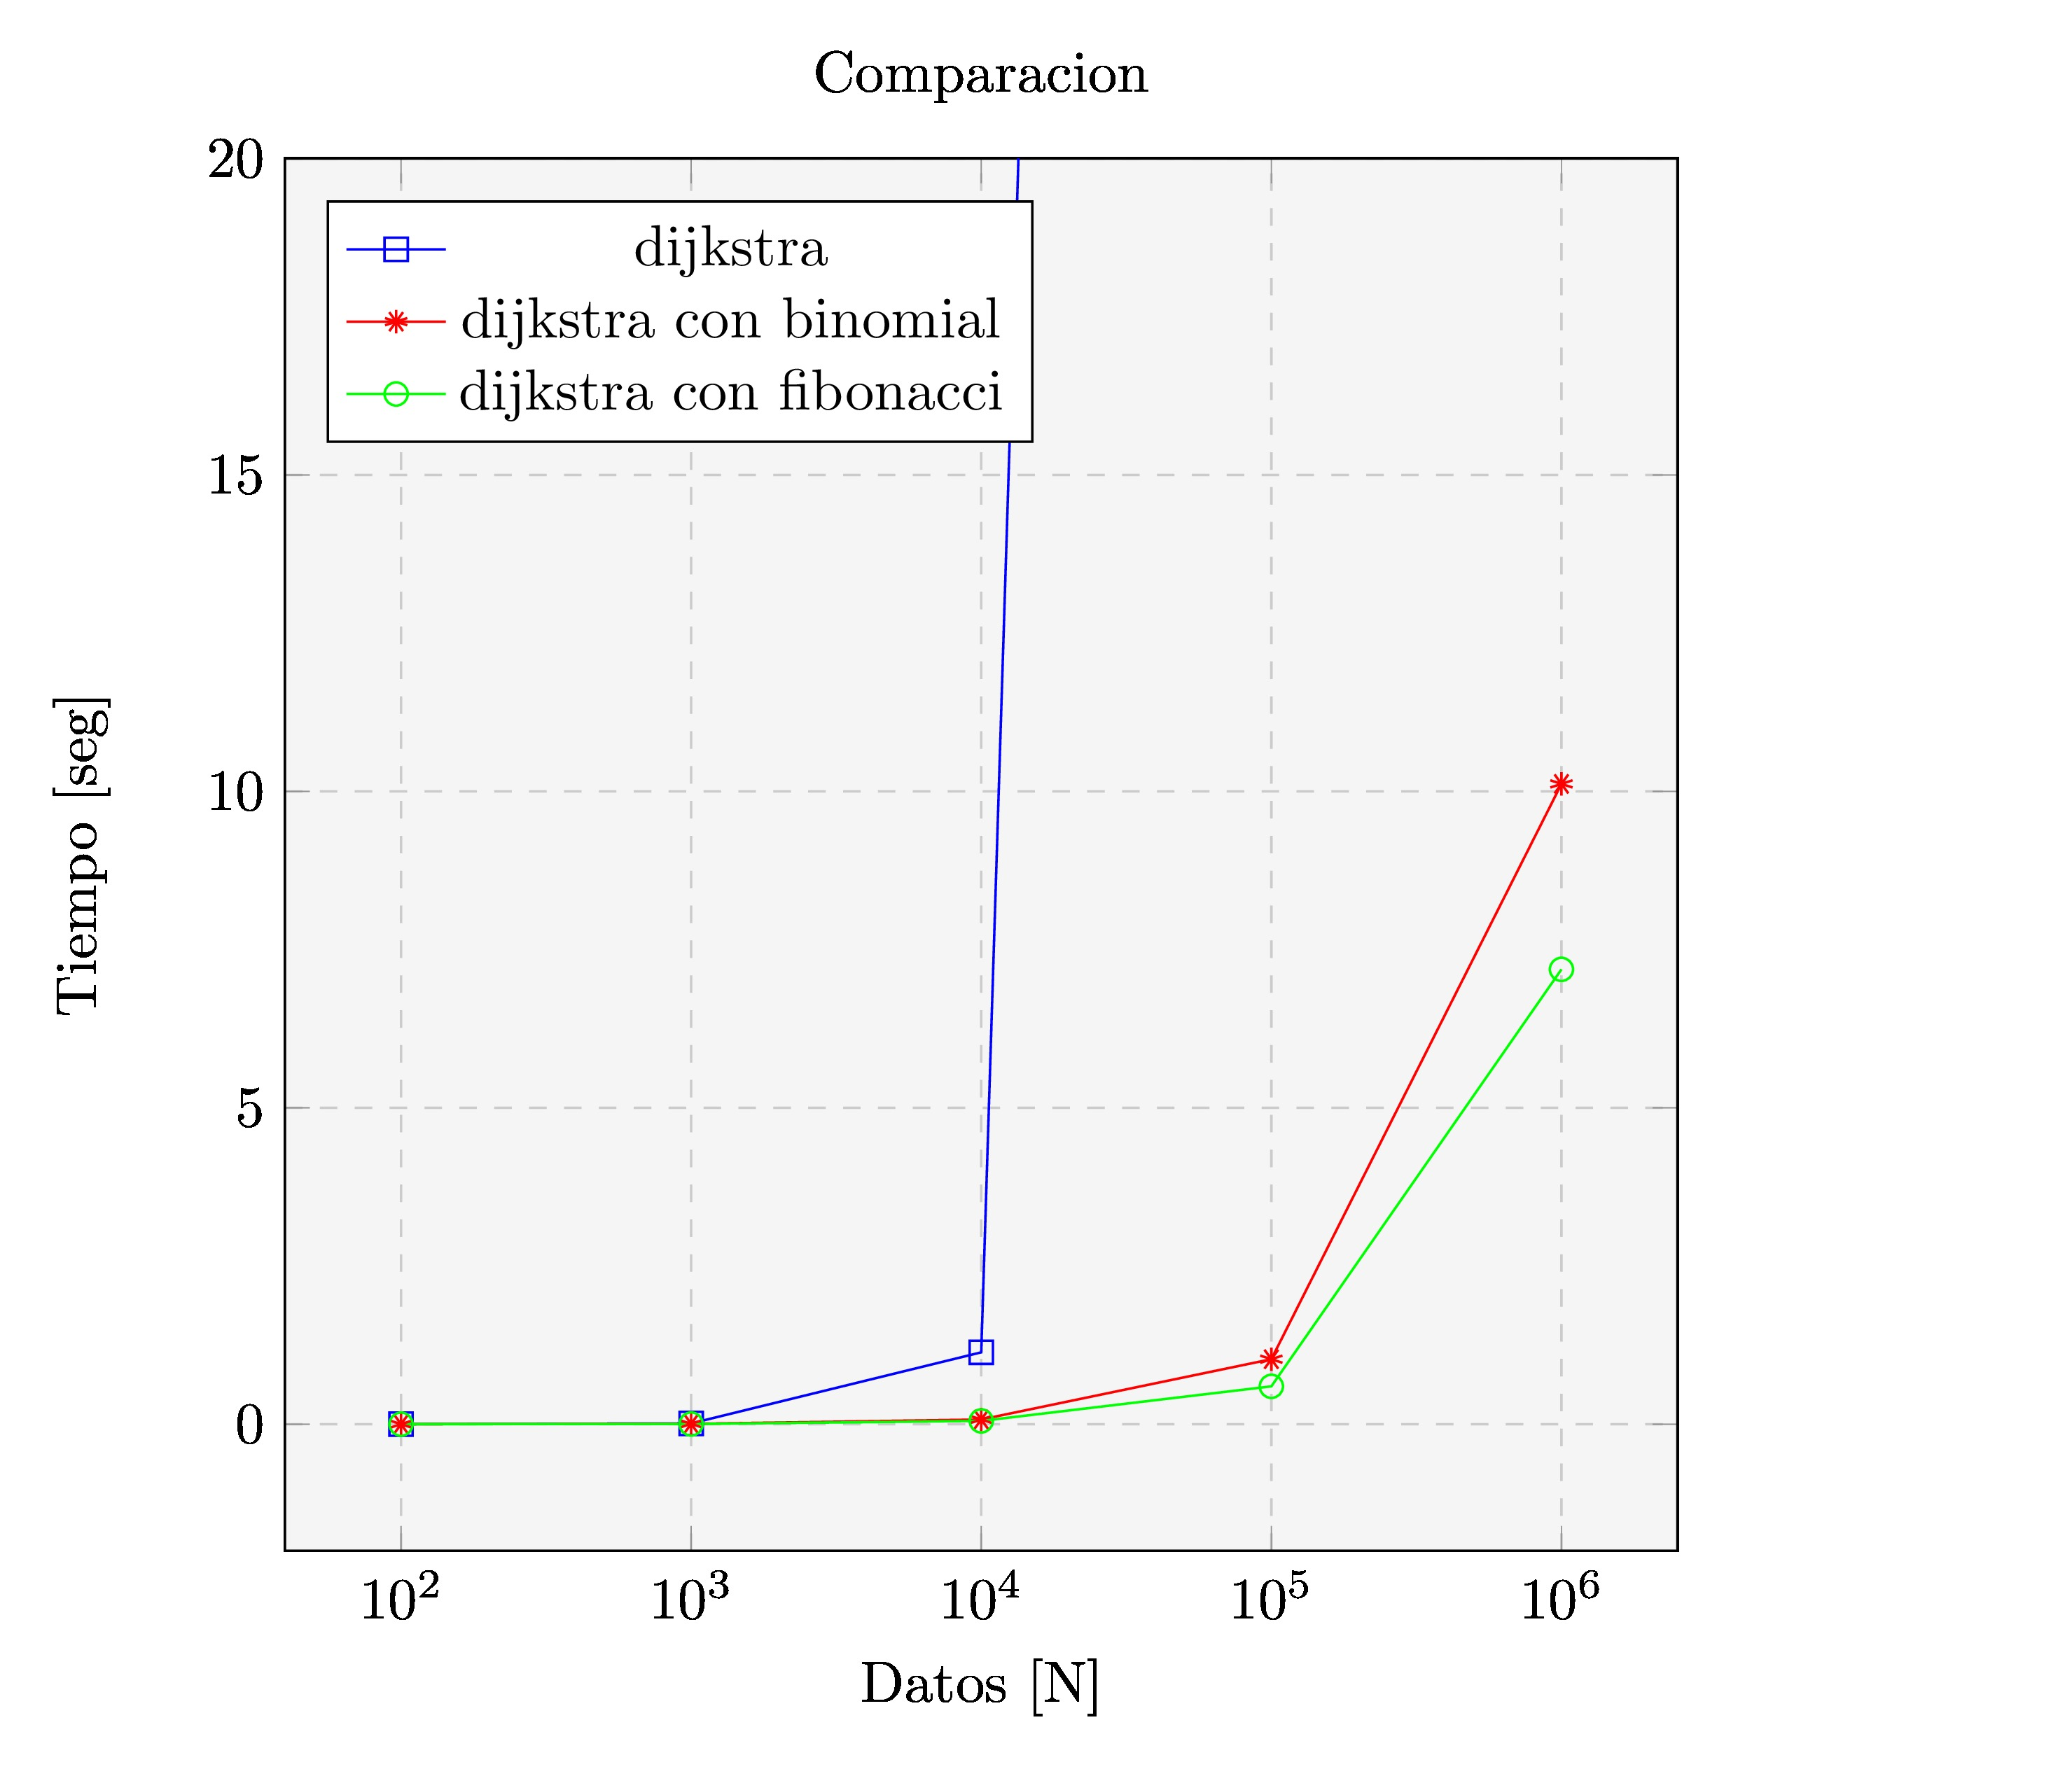
\includegraphics[width=0.7\textwidth]{graficos-3.jpg}
\end{figure}


\section{Conclusiones}
Las tres variaciones del algoritmo dijkstra poseen similar comportamiento para un grafo menor a $10^3$ nodos. Con un grafo 
mayor $10^3$ nodos la diferencianse hace notar, entre el dijkstra tradicional y los acelerados por algun heap,
Las variacones entre un Dijkstra+Binomial y un Diksjtra+Fibonacci, cobran mayor importancia en la inserción, siento el primero
de orden $0(\log(n))$ y la segunda $(1)$ en cada inserción de los nodos adyacentes en cada iteracion del $while$. Razón por 
la cual podemos concluir que para valores mayores a $10^6$ un dijkstra+Fibonacci hara notar su rapidez.


%%/////////////////////////////////////////////////////////
\begin{thebibliography}{9}
\bibitem{libro_cormen}
  Thomas H. Cormen, Charles E. Leiserson, Ronald L. Rivest, Cliford Stein.
  \emph{Introduction to Algorithms}.
  The MIT Press, Cambridge, Massachusetts,
  3rd Edition,
  2009.

\bibitem{princeton_Slides_dijkstra}
  Kevin Wayne,
  \emph{Robert Sedgewick -  Algorithms - Fourth edition}.
  Princeton University,
  2012.
  
\bibitem{princeton_slides_binomial}
  Kevin Wayne,
  \emph{Binary and Binomial Heaps - Theory of Algorithms}.
  Princeton University,
  2002.

\bibitem{princeton_slides_rezaul_dijkstraFibonacci}
  Rezaul A. Chowdhury,
  \emph{Lectures 13 y 13 (dijkstra and fibonacci heap)}.
  Department of Computer Science - SUNY Stony Brook
  2012.

\end{thebibliography}
%%/////////////////////////////////////////////////////////

\end{document}
